\documentclass{report}
\usepackage{fixlatvian}
\usepackage[utf8]{inputenc}
\usepackage{graphicx}
\usepackage{circuitikz}
\usepackage{pgfplots}
\pgfplotsset{width=10cm,compat=1.9}
 \usepackage [latvian.ticomposite]{babel}


\title{Vienkāršu elektrisku shēmu modelēšana}
\author{Ksenija Dobrovoļska REBC03}
\date{May 2018}

\begin{document}

\maketitle
\chapter{Teorētiska daļa}
\section{Ķēdes aprēķins}
Varianta aprēķins: \newline
Apliecības numurs ir 171REB108. \cite{Baltakmens} Aprēķinot pēc formulas sanāk ka V1 būs vienāds ar 108/10=10.8 V , R1 būs vienāds ar 0+1 un tas ir R1=1 Oms, un R2=8+1=9 Omi. \cite{Strazds} \newline

\begin{center}
    \begin{tabular}{|c|c|}
\hline     
     R1 & 1 Oms\\
     \hline
     R2 & 9 Oms\\
     \hline
     V1 & 10.8 V \\
     \hline
     U_{R2} & 10.8 V \\
     \hline
     U_{R1} & 9.7 V \\ 
\hline
\end{tabular}
\newline
\caption{1.1. tabula: datu tabula}
\end{center}

\begin{center}
\begin{circuitikz}[american voltages]
\draw
  (0,0) to [short] (2,0)
  to [R, l_=$R1$] (4,0)
  to [short] (4,3) 
  (0,0) to [V, l_=$V1$] (0,3) 
  to [short] (1,3) 
  to [R, l_=$R2$] (3,3)
  to [short] (4,3); 
\end{circuitikz}
\newline
\caption{1.1. zīm.: shēma ar circuitikz paķeti}
\end{center}
\newpage
 
\begin{center}
    

\begin{tikzpicture}
\begin{axis}[
    xlabel={R2},
    ylabel={UR2},
    xmin=0, xmax=50,
    ymin=8, ymax=11,
    xtick={0,10,20,30,40,50},
    ytick={9,10}
]
\addplot
    coordinates {
    (0,9)(10,9.8)(15,10.2)(20,10.3)(30,10.45)(40,10.5)(50,10.6)
    };
\end{axis}
\end{tikzpicture}
\newline
\caption{1.2. zīm.: plots ar pgfplots paķeti}
\end{center}  
  \newpage

\chapter{Praktiskā daļa}
\section{Darbs ar GEDA programmām}
\subsection{darbs ar gschem}

    \begin{figure}[!htb]
    \centering
        \includegraphics[scale=0.4]{1}
        \caption{Shēma veidota ar gschem}
    \end{figure} \newpage


\subsection{darbs ar gnetlist}
\begin{verbatim}
* Spice netlister for gnetlist
R2 2 0 9
R1 1 2 1
V1 1 0 10.8
.END
\end{verbatim}

\subsection{darbs ar ngspice}
 \begin{figure}[!htb]
    \centering
        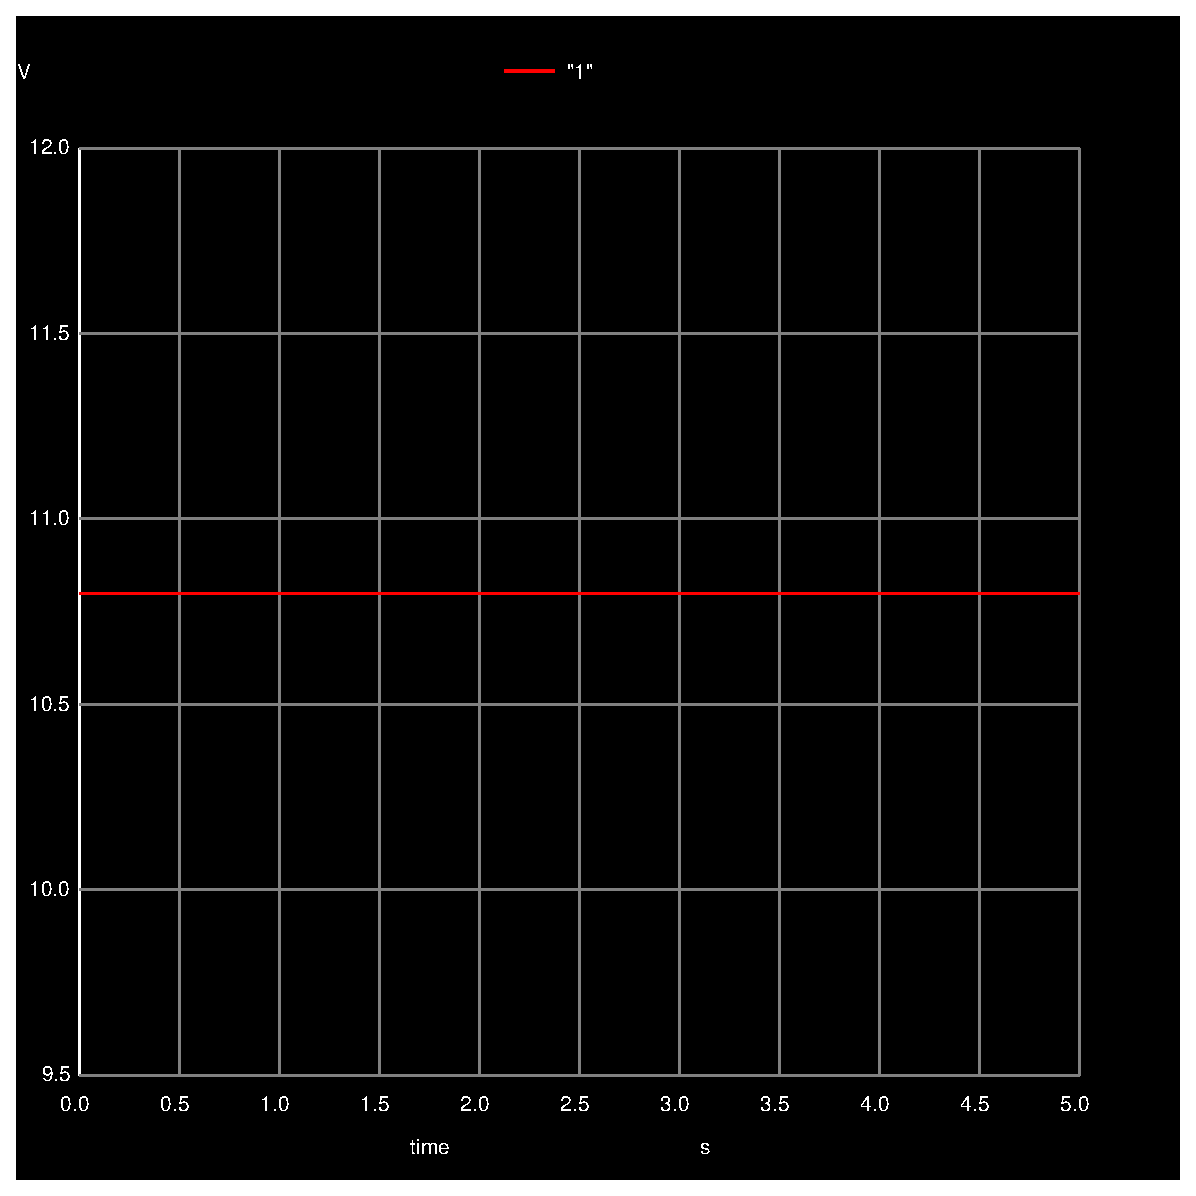
\includegraphics[scale=0.6]{011.ps}
        \caption{R1 simulācijas grafiks}
    \end{figure} \newpage
    
     \begin{figure}[!htb]
    \centering
        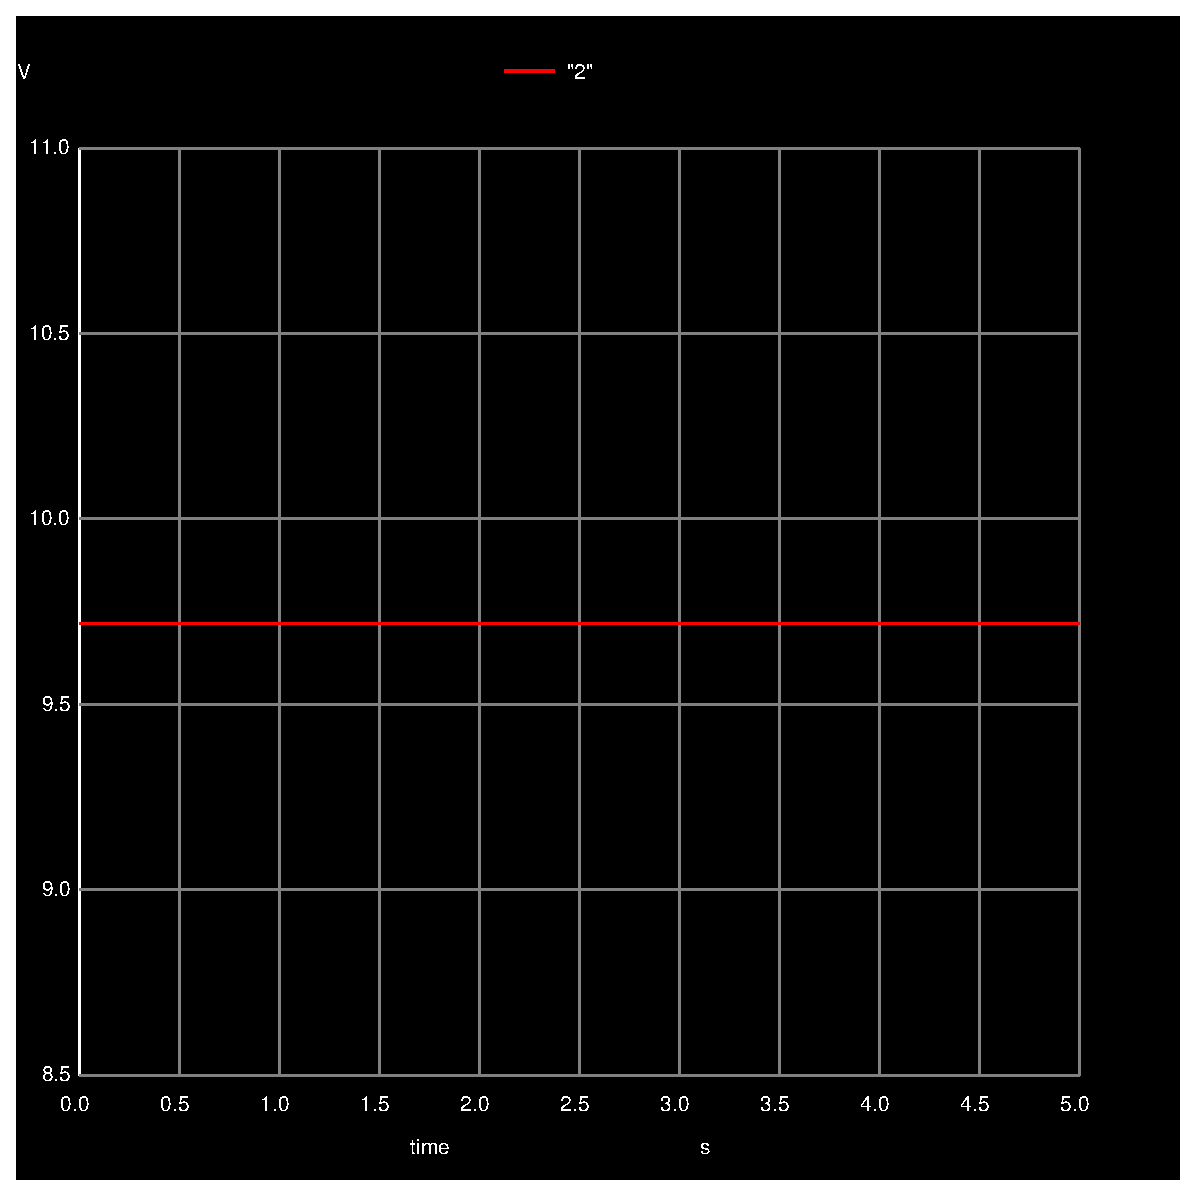
\includegraphics[scale=0.6]{012.ps}
        \caption{R2 simulācijas grafiks}
    \end{figure} \newpage



\section{Darbs ar QUCS programmām}

    \begin{figure}[!htb]
    \centering
        \includegraphics[scale=0.5]{2}
        \caption{Shēma QUCS vidē}
    \end{figure}


    \begin{figure}[!htb]
    \centering
        \includegraphics[scale=0.5]{kq1}
        \caption{Sweep simulacija}
    \end{figure}
    
    \begin{figure}[!htb]
    \centering
        \includegraphics[scale=0.5]{kq2}
        \caption{Sweep grafiks/tabula}
    \end{figure}
\newpage
\renewcommand{\bibname}{Literatūras saraksts}
\begin{thebibliography}{9}
\bibitem{Baltakmens} 
3. Baltakmens, [\textit{R. Latvietis un viņa zirgi}]. Rīga: Valters un Rapa, 2000. 282 lpp. ISBN 9984-59-540-4

 
\bibitem{Strazds}
Strazds, M. (red.) [\textit{Latvijas ūdeņu putni}]. Rīga: Jāņa sēta, 1999. 208 lpp. ISBN 9984-9180-4-1

 
\end{thebibliography}

\end{document}
